\item Analizar en cada caso si el conjunto el linealmente independiente y hallar el subespacio generado por cada uno de ellos. Decir además qué dimensión tiene cada subespacio.
    \begin{enumerate}
        \item $B=\{(2,0,1);(3,1,2);(1,1,1);(7,3,5)\}\subset\R^3$
            \begin{mdframed}[style=s]
                Del ejercicio 4, se deduce que $B$ es un conjunto linealmente dependiente. Sea $v\in B$
                \begin{center}
                    $v=x_1(2,0,1)+x_2(3,1,2)+x_3(1,1,1)+x_4(7,3,5)\quad x_1,x_2,x_3,x_4\in\R$\\
                    $v=(2x_1+3x_2+x_3+7x_4,x_2+x_3+3x_4,x_1+2x_2+x_3+5x_4)$\\
                \end{center}
                Manipulando la expresión:
                \begin{center}
                    $v=(x_2+x_3+3x_4)(1,1,1)+(x_1+x_2+2x_4)(2,0,1)$
                \end{center}
                Se puede ver que $v$ es una combinación lineal de $(1,1,1)$ y $(2,0,1)$. En la Figura 5, se pueden observar los 4 vectores de $B$ y el plano en el que están contenidos
                \begin{center}
                    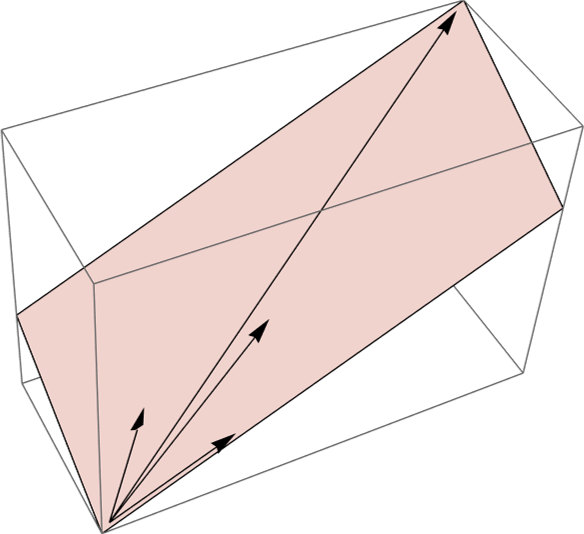
\includegraphics[width=0.4\textwidth]{Ej8.png}\\
                    Figura 5. Espacio generado por un conjunto de vectores.
                \end{center}
                El plano que generan se puede encontrar haciendo el producto vectorial entre los vectores generadores y se obtiene $\pi:x+y-2z=0$. Como generan un plano, la dimensión del espacio generado es 2.
            \end{mdframed}
        \item $B=\left\{\begin{pmatrix}
                2&1\\0&0
            \end{pmatrix};\begin{pmatrix}
                0&0\\2&1
            \end{pmatrix};\begin{pmatrix}
                3&-1\\0&0
            \end{pmatrix}\right\}\subset\R^{2\times2}$
            \begin{mdframed}[style=s]
                $x_1\begin{pmatrix}
                    2&1\\0&0
                \end{pmatrix}+x_2\begin{pmatrix}
                    0&0\\2&1
                \end{pmatrix}+x_3\begin{pmatrix}
                    3&-1\\0&0
                \end{pmatrix}=\begin{pmatrix}
                    0&0\\0&0
                \end{pmatrix}\to \begin{cases}
                    2x_1+3x_3=0\\
                    x_1-x_3=0\\
                    2x_2=0\\
                    x_2=0
                \end{cases}\to x_1=x_2=x_3=0$\\
                Por lo tanto, $B$ es un conjunto linealmente independiente, entonces
                \begin{center}
                    $\overline{B}=\overline{\left\{\begin{pmatrix}
                        2&1\\0&0
                    \end{pmatrix};\begin{pmatrix}
                        0&0\\2&1
                    \end{pmatrix};\begin{pmatrix}
                        3&-1\\0&0
                    \end{pmatrix}\right\}}$.
                \end{center}
                También se puede pensar en que el espacio generado está compuesto por matrices de la forma
                \begin{center}
                    $A=\begin{pmatrix}
                        a&b\\2d&d
                    \end{pmatrix}\quad a,b,d\in\R$
                \end{center}
                Es decir, 
                \begin{center}
                    $\overline{B}=\left\{\begin{pmatrix}
                        a_{11}&a_{12}\\a_{21}&a_{22}
                    \end{pmatrix}\in\R^{2\times2}:2a_{22}=a_{21}\right\}$    
                \end{center}
                Por último, dim$(\overline{B})=3$
            \end{mdframed}
        \item $B=\{1-x,2-x^2,x+x^2\}\subset\R_2[x]$ (el conjunto de polinomios de grado menor o igual a 2 con coeficientes en $\R$).
            \begin{mdframed}[style=s]
                \begin{center}
                    $\alpha(1-x)+\beta(2-x^2)+\gamma(x+x^2)=0\to\begin{cases}
                        \alpha+2\beta=0\\
                        -\alpha+\gamma=0\\
                        -\beta+\gamma=0
                    \end{cases}\to \alpha=\beta=\gamma=0\to$ son li.
                \end{center}
                Como son 3 polinomios li de un espacio de dimensión 3, generan a $\R_2[x]$.
            \end{mdframed}
    \end{enumerate}
    